\begin{mdframed}[style=warning]
	\textbf{Conceptos}
		\begin{enumerate}
			\item Distinga claramente entre temperatura, calor y energía interna.
			\item Con la primera ley de la termodinámica explique por qué la energía total de un sistema aislado siempre es constante.
		\end{enumerate}
\end{mdframed}


















\begin{mdframed}[style=warning]
	\begin{ejercicio}
		Padeciendo la gripe una persona de $80kg$ tuvo una fiebre de $39^o C$. La temperatura normal de cuerpo humano es de $36.6^o C$. Suponemos que el cuerpo humano es agua en su mayor parte, y suponemos que la persona recuperó su temperatura normal gracias sólo a la sudoración.
		\begin{enumerate}
			\item ¿Cuánta energía se necesitó para elevar la temperatura del enfermo?
			\item ¿Cuánto sudor se evaporó de su cuerpo para enfriarse?
		\end{enumerate}
		{\textit{Datos: Calor específico del agua $c_{H_2 O} = 41.87 J/kg*^o C$; calor latente de vaporización (a la temperatura de la piel) $L = 2416 kJ/kg$; densidad $1000 kg/m^3$.}}
	\end{ejercicio}
\end{mdframed}




















\begin{mdframed}[style=warning]
	\begin{ejercicio}
		En un tbo vertical liso abierto por ambos extremos y con secciones diferentes arriba y abajo se encuentran dos émbolos, unidos por un hilo inalargable, y entre los émbolos, un mol de gas perfecto (ideal). El área del émbolo superior es $\Delta S = 10cm^2$ mayor que la del inferior. La masa total de los émbolos $m = 5kg$. La presión atmosférica $p_o$. ¿En cuántos grados Kelvin debe calentarse el gas contenido entre los émbolos, para que éstos se desplacen l = $5cm$?
		\begin{figure}[H]
			\centering
			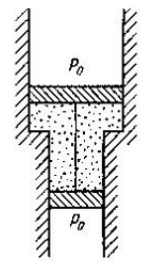
\includegraphics[scale=0.5]{./img/embolo.png}
			\label{embolo}
		\end{figure}
	\end{ejercicio}
\end{mdframed}













\begin{mdframed}[style=warning]
	\begin{ejercicio}
		Un cilindro vertical de radio $r$ contiene una cantidad de gas ideal, y está provisto de un pistón con masa $m$ que puede moverse libremente. El pistón y las paredes del cilindro carecen de fricción, y el cilindro, y el cilindro completo se coloca en un baño a temperatura constante. La presión del aire exterior es $p_o$. En equilibrio, el pistón está a una altura $h$ sobre la base del cilindro. $a)$ Calcule la presión absoluta del gas atrapado bajo el pistón cuando está en equilibrio. $b)$ Se tira el pistón para subirlo una distancia corta  y después se suelta. Determine la fuerza neta que actúa sobre el pistón cuando su base está a una distancia $h + y$ sobre la base del iclindro, donde $y$ es mucho menor que $h$. $c)$ Después de que el pistón se desplaza del equilibrio y se suelta, oscila verticalmente. Calcule la frecuencia de estas pequeñas oscilaciones. Si el desplazamiento no es pequeño, ¿las oscilaciones son armónicas simples? ¿Cómo lo sabe?
		\begin{figure}[H]
			\centering
			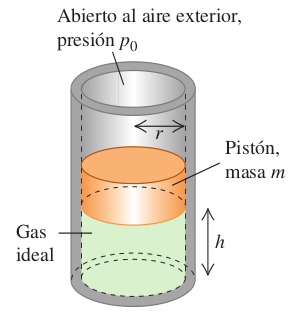
\includegraphics[scale=0.45]{./img/piston.png}
			\label{embolo}
		\end{figure}
	\end{ejercicio}
\end{mdframed}


















\begin{mdframed}[style=warning]
	\begin{ejercicio}
		Un lanzador de papas dispara una papa de forma horizontal a través de un cilindro con tapa cerrada y sección transversal $A$. La papa inicialmente está en reposo y el volumen entre esta y la parte cerrada del cilindro es $V_o$. La presión inicial es $P_o$. La presión atmosférica es $P_{atm}$, donde $P_o > P_{atm}$. El gas en el cilindro es diatómico, lo que significa que $C_V = 5R/2$ y $C_p = 7R/2$. La papa se mueve sin fricción y no hay filtraciones de gas en el sistema. Los parámetros $P_o$, $P_{atm}, V_o$ y $A$ están fijos, pero el largo $L$ puede variar.
		\begin{enumerate}
			\item ¿Cómo debe de ser la relación entre las presiones para que la energía de la papa sea mayor posible al momento de salir del tubo?
			\item Si no hay una fuente externa de calor ¿Qué tipo de proceso termodinámico se tiene?
			\item En base a esta información ¿Cuál es la energía cinética máxima que puede adquirir la papa cuando sale del cilindro? Para este caso ¿Cuál es la longitud L? Expresar las respuestas en términos de $P_o$, $P_{atm}$ y $V_o$.
		\end{enumerate}
	\end{ejercicio}
\end{mdframed}




















%%%